\section{Introduction}
\label{sec:intro}

Algorithms for the detection of manipulated content in digital images have reached a stage of maturity that is sufficient for understanding the transformations that were applied to individual images in many cases~\cite{farid2009image,Rocha:CSUR:2011,farid2017detect}.
A logical next step is to develop an approach that allows us to ask more complicated questions about the relationships between related images after sequences of transformations have been applied --- a problem that is not well studied in the image processing literature.
In this article, we consider the \textit{Provenance Analysis} task~\cite{Dias_2012,Dias_2013}, in which the objective is to recover the graph of relationships between plausibly connected images. These relationships may be expressed as undirected edges (\textit{i.e.}, neighboring transformations are identified) or directed edges (\textit{i.e.}, the order of neighboring transformations is expressed).
The development of techniques to recover such graphs combines ideas from the areas of image retrieval, digital image forensics, and graph theory, making this an interesting interdisciplinary endeavour within image processing and computer vision. 

%(Teaser Figure; meme example)
\begin{figure}[t]
\centering
\vspace{-0.3cm}
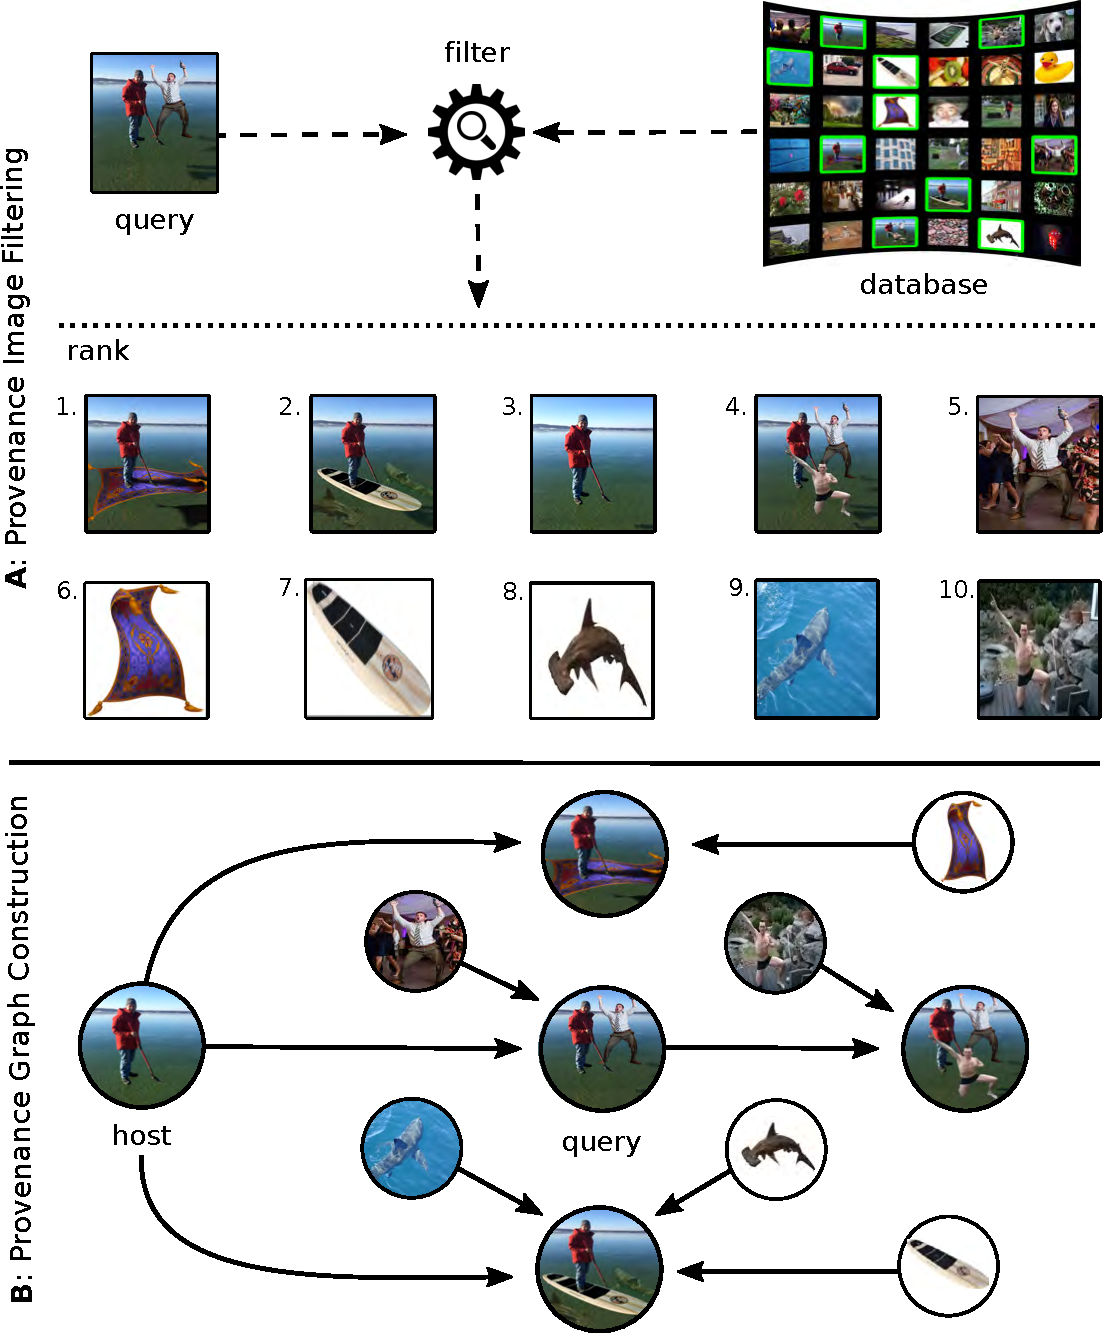
\includegraphics[width=8.7cm]{figures/teaser7.pdf}
\caption[Image Provenance Analysis]{Image Provenance Analysis workflow.
Panel A depicts the first step of Image Provenance Analysis, namely Provenance Image Filtering, in which filters are applied to a large image database to retrieve those images that are related to a given query image.
Panel B depicts the second step, namely Provenance Graph Construction, in which the filtered images are linked to each other in a way that expresses the sequences of manipulation and/or compositions (\textit{i.e.}, the provenance history of the images).}
%\vspace{-0.2cm}
\label{fig:teaser}
\end{figure}

%In more concrete terms, what is the provenance analysis task?
To illustrate the provenance analysis task, consider the set of example images in Panel A of Fig.~\ref{fig:teaser}, which were collected from the popular ``Photoshop battles'' forum on the social media site Reddit~\cite{reddit2017photoshopbattles}.
On this forum, amateur artists begin with source images and employ image manipulation tools to generate results for humorous effect.
The first step in provenance analysis is \textit{Provenance Image Filtering}, which consists of searching a potentially large pool of images for those that are most closely related to a given query image.
Related images might be {\em semantically similar} ({\em i.e.}, the same scene may be present from slightly different view points or at nearby points in time), or they might be {\em near duplicates} related by minor transformations such as exposure and saturation adjustments, or cropping and re-sizing, or they might be {\em  image compositions}, which contain elements of two or more different source images.
In most cases, the query will be an image that has been manipulated in some way. 

The second step is \textit{Provenance Graph Construction}, where the objective is to understand the relationships between images yielded by provenance image filtering.
A \textit{Host Image} provides the source of background content for subsequent manipulations.
In Fig.~\ref{fig:teaser}, the host is the photo of the man holding a shovel in the 
leftmost part of Panel B. % (itself a likely copy-move forgery~\cite{fridrich2003detection}).
A \textit{Donor Image} provides some amount of content that will be inserted into a host image.
In Fig.~\ref{fig:teaser}, three donor images are the original images of the sharks and the paddle board in the %center 
bottom half of Panel B.
They provide image content that has been inserted into the image %to their left
they are linked to.
Sequences of manipulations are common, and they can be expressed as a directed graph representing the order in which they were applied.
This can be seen in the %overall graph in Panel B,
graph of Panel B, where the depth %of certain paths
of the central path containing the host and the query 
leads to three different levels of manipulations.
Our goal %in this work
is to develop an algorithm that can generate such graphs in an automated fashion.
We do not make strong assumptions that either the original host or donor images are available during analysis. %For instance, the surfboard, magic carpet, elephant, and extra people were not harvested at the image retrieval stage of the process.
For instance, the paddle board, flying carpet, and extra people might not necessarily be harvested at the image filtering step.
% In addition, the analysis does not have any restriction on the number and type of unrelated images (distractors) to be assessed in a potential pool of images

%Why is provenance analysis important to image processing?
Provenance analysis is important to image processing and computer vision.
%This problem is not posed as just a thought experiment.
%On the contrary,
It has direct applications in a number of different fields.
The most immediate application is forensics, where the detection of manipulated images spans traditional policing to analysis for strategic intelligence.
The question of the origins of suspect images has taken a prominent role recently, with the rise of so-called ``fake news" on the Internet. 
While not a new problem\footnote{The computer hacker group Cult of the Dead Cow warned of the devastating potential of widespread online media manipulation as early as 1999~\cite{cdc}.}, concern about fake news reached new heights on the heels of the 2016 American presidential election.
The rapid evolution of the online social media landscape has provided new, free media channels with which even amateur bloggers and news outlets can reach massive audiences with little effort, and even less regulation.
Recent instances of fake news often involve questionable images propagating through social media.
For example, in early 2017, the New York Times reported on the creation of a false story about the discovery of pre-marked ballots in Ohio that appeared a couple of months before the election~\cite{NYT1}.
The image accompanying the story was the product of a mirrored image that was selectively blacked-out in local regions~\cite{PP1}.
This is a real-life case with multiple manipulations where provenance analysis could be applied to trace the origins of the fabrication. 
% Expert analysis cannot feasibly be deployed to the massive influx of data that bombards average internet users on a daily basis, such as the article above. Unfortunately, users tend resonate with stories and media that appeal to them emotionally and viscerally \cite{pronin2007valuing}. 

%% Probably out of scope for this paper
%%A related application is plagiarism / scientific %misconduct detection. (cite) Where  the content came from %can shed some light on the case.

Beyond the important application domain of forensics, image provenance analysis can form a powerful framework for academic research in other fields.
Cultural analytics has emerged as a distinct sub-discipline within the digital humanities~\cite{manovich2009cultural,yamaoka2011cultural} that is concerned with combining quantitative methods from social science and computer science to answer humanistic questions about cultural trends.
An example of this (which we have already touched upon in Fig.~\ref{fig:teaser}) is the study of Internet \textit{memes} --- cultural artifacts meant to be widely transmitted and evolve over time.
Memes are an interesting object of cultural study, in that they encapsulate facets of popular entertainment, political moods, and novel elements of humor.
Meme aggregators like the website \emph{knowyourmeme.com} have done a good job at archiving such content, but a more exhaustive quantitative study of the provenance of individual memes has yet to emerge.
Tracing the source(s) of modified meme images helps us unpack the underlying cultural trends that can tell us something meaningful about the community that generated the content.



%% What algorithmic components are necessary to solve this problem?
%% First, one needs an accurate and scalable image retrieval algorithm that is able to operate over very large collections of images (realistically, on the order of millions of images) to find related candidates.
%% Second, identification of image transformations and the localization of any tampering provide evidence for the ordering of the related images.
%%And third, methods from graph theory are necessary to establish the relationships between images, yielding a directed graph that is interpretable by a human analyst.
%% Further, all of these components must be integrated to solve the problem as a coherent processing pipeline.
%What algorithmic components are necessary to solve this problem?
Both of the application domains mentioned also motivate the need for any developed techniques to be {\em scalable}.
Specialized algorithmic components are necessary to solve the problem at hand.
First, one needs an accurate and scalable image retrieval algorithm that is able to operate over very large collections of images (realistically, on the order of millions of images) to find related candidates.
Such an algorithm also has to address the particularities of the provenance image filtering task: it must perform well at retrieving the near-duplicate host images that are highly related to the query (a well-known problem in the image retrieval literature), but also perform well at retrieving donors (images that potentially donated small portions to the query) and the donors' respective near duplicates (which might not be directly related to the query).
Second, the identification of likely image transformations that explain how each retrieved image might have been used to generate the others is required, as it is used to create the ordering of the images in the provenance graph.
And third, methods from graph theory are necessary to organize the relationships between images, yielding a directed graph that is human-interpretable. % by a human analyst.
All of these components must be integrated %to solve the problem
as a coherent and scalable processing pipeline.

%% The components of the pipeline rely on existing algorithms (and some of the possible choices, like those in the area of image retrieval, are fairly mature technologies), but there is significant need for further work to support the specific objective of provenance analysis. The scale of the filtering. Shih-fu? Us. Recent methods based on deep learning are not good for this. Trade-off in speed versus accuracy for dense feature extraction. Manipulated regions of images are often highly localized. Need to identify where and target those regions and incorporate the context. The existing literature focuses on undirected graphs. Extend to establish directions within the graph.
%%
%Along these lines, the contributions of this article are:
%%\begin{enumerate}
%%    \item A novel provenance image filtering technique that is able to scale to over a million images.
%%    \item A novel un-directed graph construction algorithm that is able to find a relationship map for a set of images.
%%    \item A novel directed graph construction algorithm that is able to infer the order of transformations applied to related images.
%%    \item State-of-the-art results on a newly released benchmark (cite) designed specifically for provenance analysis.
%%    \item A new dataset of real images from photoshop battles held on the website Reddit. Experiments performed over this dataset highlight the real-world applicability of the approach.
%%\end{enumerate}

%How does this work contribute to solving the problem?
%Besides putting together, for the first time, a fully automated large-scale end-to-end pipeline that starts with the initial step of provenance image filtering (over millions of images) and ends up with the provenance graphs, this article introduces:

% [MAJOR] Moved to the end of related work >>>>>>>
%This work introduces, for the first time, a fully automated large-scale end-to-end pipeline that starts with the step of provenance image filtering (over millions of images) and ends up with the provenance graphs.
%The following new contributions are introduced this work:
%
%\vspace{0.2cm}
%\begin{enumerate}
%\item \emph{Distributed interest point selection}: a novel interest point selection strategy that aims at spatially diversifying the image regions used for indexing within the provenance image filtering task.
%
%\item \emph{Iterative Filtering}: a novel querying strategy that iteratively retrieves images that are  directly or indirectly related to the query, considering all possible hosts, donors, composites, and their respective near duplicates.
%
%\item \emph{Clustered Provenance Graph Construction}: a novel graph construction algorithm that clusters images according to their content (joining near duplicates into the same clusters), prior to establishing their intra- and inter-cluster relationship maps.
%
%\item State-of-the-art results on the provenance analysis benchmark released by the American National Institute of Standards and Technology (NIST)~\cite{nist2017dataset}.
%
%\item A new dataset of real-world scenarios containing composite images from Photoshop battles held on the Reddit website~\cite{reddit2017photoshopbattles}.
%Experiments performed over this dataset highlight the real-world applicability of the approach.
%\end{enumerate}
% <<<<<<< [MAJOR] Moved to the end of related work
\RED{In this context, this work introduces, for the first time, a fully automated large-scale end-to-end pipeline that starts with the step of provenance image filtering (over millions of images) and ends up with the provenance graphs.}

% Cut for space. WJS
%In the rest of this article, we explain what a practical end-to-end pipeline for provenance analysis looks like.
%In the rest of this article, we explain how the proposed %end-to-end pipeline for provenance analysis looks like.
%In Sec.~\ref{sec:rw}, we review the relevant literature %in this emerging area of image processing, highlighting %the advances made by existing approaches, as well as %their current weaknesses.
%Then, in Sec.~\ref{sec:prop}, we introduce methods for %provenance image filtering and graph construction.
%Aiming at assessing the performance of the proposed %solutions, a experimental setup is described in %Sec.~\ref{sec:expsetup}, while its results are reported %in Sec.~\ref{sec:results}.
%Finally, we provide some conclusions and discuss future %work in Sec.~\ref{sec:conc}.
